\documentclass{article}
\usepackage[T1]{fontenc}
\usepackage{titlesec}
\usepackage{graphicx}
\usepackage{amsmath}
\usepackage{xcolor}
\titleformat{\section}  % which section command to format
  {\fontsize{10}{12}\bfseries} % format for whole line
  {\thesection} % how to show number
  {1em} % space between number and text
  {} % formatting for just the text
  [] % formatting for after the text
\title{Logika Cyfrowa}
\author{Jakub Gałaszewski} 
\begin{document}
\maketitle
\section{ Za pomocą przekształceń algebry Boole’a znajdź najmniejsze wyrażenie w dysjunkcyjnej postaci normalnej równoważne $x\bar{y}\bar{z} + xyw + x\bar{y}z\bar{w}$.}
 \textbf{dysjunkcyjna postać normalna} inaczej DNF to alternatywa koniukcji literałów.\\
 $x\bar{y}\bar{z} + xyw + x\bar{y}z\bar{w}=x\bar{y}(\bar{z}+z\bar{w}) + xyw=x\bar{y}(\bar{z}+\bar{w}) + xyw = x\bar{y}\bar{z} + x\bar{y}\bar{w} + xyw$\\
 $X+\bar{X}Y = X(1+Y)+ \bar{X}Y = X + Y(X + \bar{X})=X+Y$
\section{a pomocą przekształceń algebry Boole’a znajdź najmniejsze wyrażenie w koniunkcyjnej postaci normalnej równoważne $(x + z + w)(x + \bar y + z)(x + \bar y + \bar z + w)$.}
 \textbf{koniunkcyjna postać normalna} inaczej CNF to koniukcja alternatyw literałów.\\
 $(x + z + w)(x + \bar y + z)(x + \bar y + \bar z + w) = x+(z + w)(\bar y + z)(\bar y + \bar z + w) = x+(z + w) (\bar y + z(\bar z + w)) =x+(z + w)(\bar y + zw)  = x+(z + w)(\bar y + z)(\bar y + w) = (x+z + w)(x + \bar y + z)(x + \bar y + w)$
 \section{zaprojektuj najprostszy obwód typu suma iloczynów implementujący funkcję $f (x, y, z) = \sum m(1, 3, 4, 6, 7)$}
 skorzystam z tabeli Karnaugh'a w celu określenia minimalnej sumy iloczynów:
 \begin{center}
	\begin{tabular}{|c||c|c|c||c|} 
	 \hline
	$n$ & $x$ & $y$ & $z$ & $\phi$\\ 
	 \hline \hline
	 0&0&0&0&0\\ \hline
	 1&0&0&1&1\\ \hline
	 2&0&1&0&0\\ \hline
	 3&0&1&1&1\\ \hline
	 4&1&0&0&1\\ \hline	 
	 5&1&0&1&0\\ \hline
	 6&1&1&0&1\\ \hline
	 7&1&1&1&1\\ \hline
	\end{tabular}
	\begin{tabular}{|c|c|c|c|c|} 
	 \hline
	x \textbackslash yz& 00 & 01 & 11 & 10\\ 
	 \hline
	 0&0&1&1&0\\ \hline
	 1&1&0&1&1\\ \hline
	\end{tabular}\\
	$\phi = \bar x z + xy + x \bar z$\\
	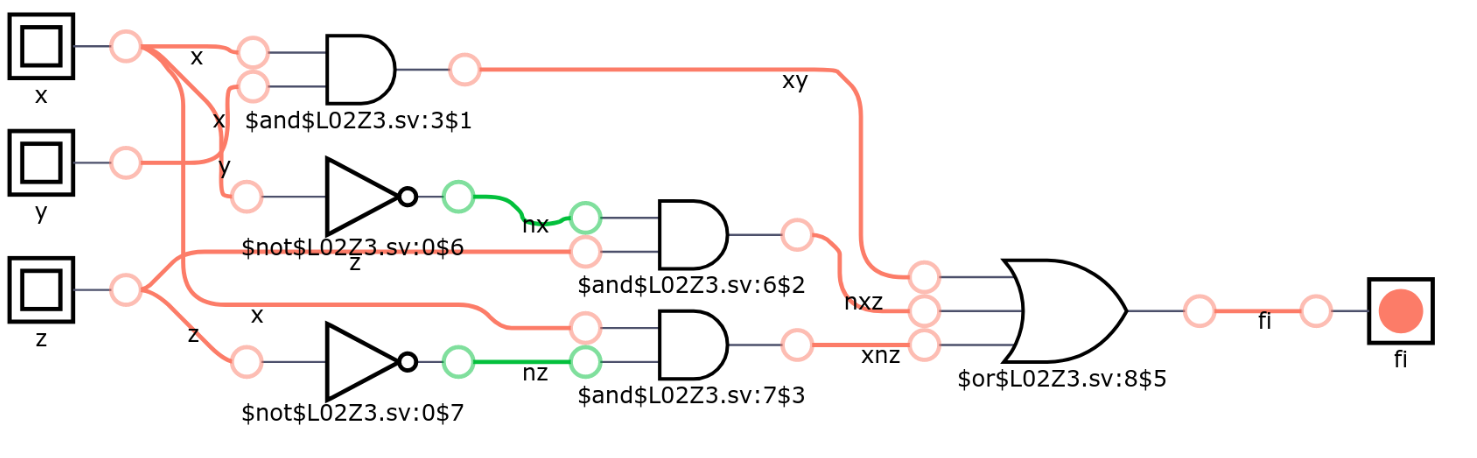
\includegraphics[scale=0.3]{./L02Z03.png}
	\textbf{można złapać prościej:}
	\begin{tabular}{|c|c|c|c|c|} 
	 \hline
	x\textbackslash yz& 00 & 01 & 11 & 10\\ 
	 \hline
	 0&0&\textcolor{red}1&\textcolor{red}1\textbackslash \textcolor{blue}1&0\\ \hline
	 1&\textcolor{green}1&0&\textcolor{blue}1&\textcolor{green}1\\ \hline
	\end{tabular}\\
	$\phi = x\bar{z} + zy + \bar{x}z$\\
		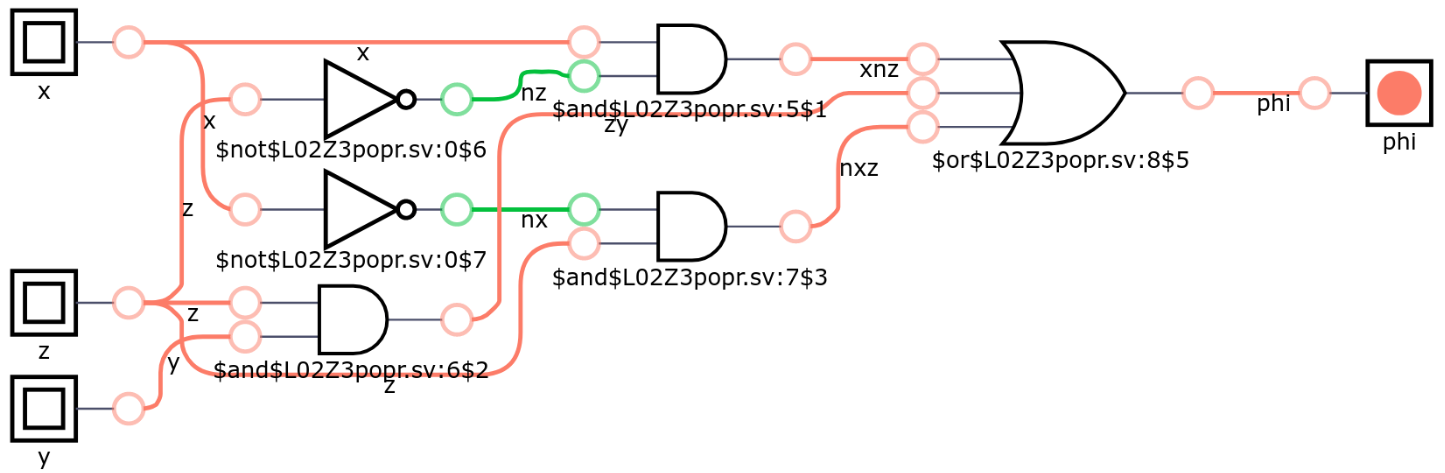
\includegraphics[scale=0.3]{./L02Z03popr.png}
\end{center}
\section{Zaprojektuj najprostszy obwód typu iloczyn sum implementujący funkcję $f (x, y, z) = \prod M (0, 2, 5)$.}
 \begin{center}
	\begin{tabular}{|c||c|c|c||c|} 
	 \hline
	$n$ & $x$ & $y$ & $z$ & $\phi$\\ 
	 \hline \hline
	 0&0&0&0&0\\ \hline
	 1&0&0&1&1\\ \hline
	 2&0&1&0&0\\ \hline
	 3&0&1&1&1\\ \hline
	 4&1&0&0&1\\ \hline	 
	 5&1&0&1&0\\ \hline
	 6&1&1&0&1\\ \hline
	 7&1&1&1&1\\ \hline
	\end{tabular}
	\begin{tabular}{|c|c|c|c|c|} 
	 \hline
	x \textbackslash yz& 00 & 01 & 11 & 10\\ 
	 \hline
	 0&0&1&1&0\\ \hline
	 1&1&0&1&1\\ \hline
	\end{tabular}\\
	$ \phi = (x+y+z)(\bar x +y+ \bar z)(x + \bar y + z)$\\
	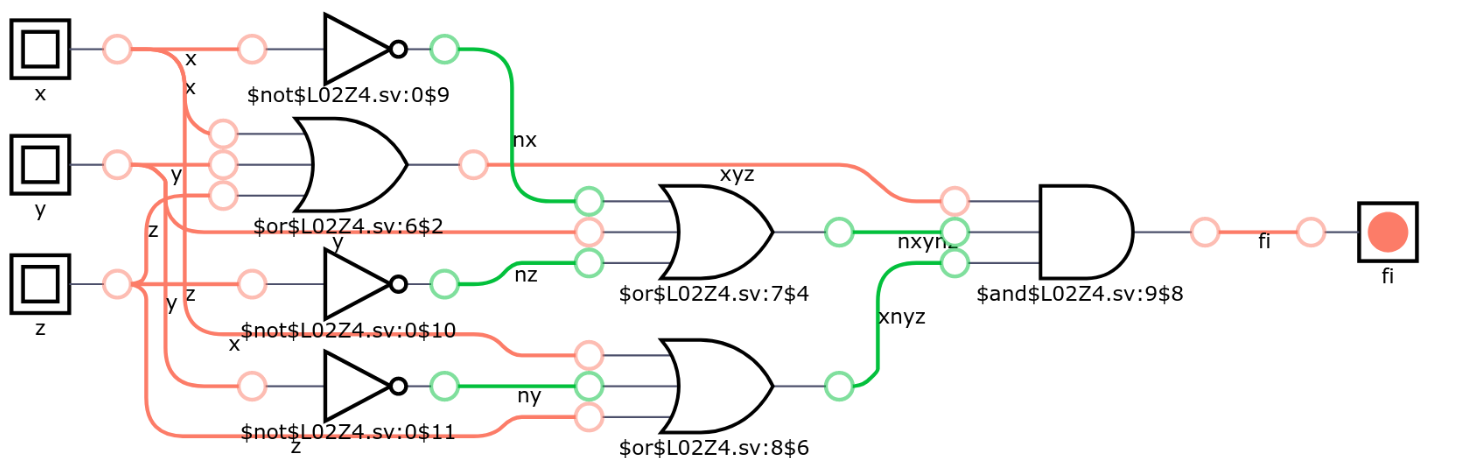
\includegraphics[scale=0.3]{./L02Z04.png}
	\textbf{można prościej:}
	$ \phi = (x+z)(\bar{x} + y + \bar{z})$\\
	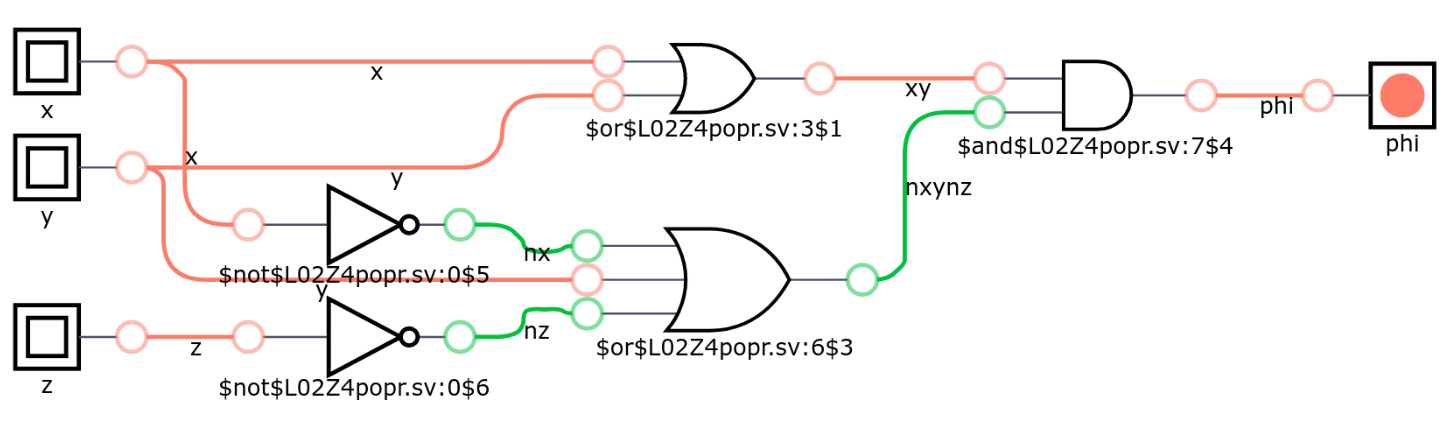
\includegraphics[scale=0.3]{./L02Z04popr.png}
\end{center}
\section{Zaprojektuj najprostszy obwód o trzech wejściach i jednym wyjściu, który produkuje wyjście 1 wtedy i tylko wtedy, gdy dokładnie jedno lub dwa wejścia mają wartość 1, w przeciwnym wypadku produkuje wyjście 0.}
\begin{center}
\begin{tabular}{|c|c|c|c|c|} 
	 \hline
	x \textbackslash yz& 00 & 01 & 11 & 10\\ 
	 \hline
	 0&0&1&1&1\\ \hline
	 1&1&1&0&1\\ \hline
	\end{tabular}\\
	$\phi = (x+y+z)(\bar x + \bar y + \bar z)$\\
	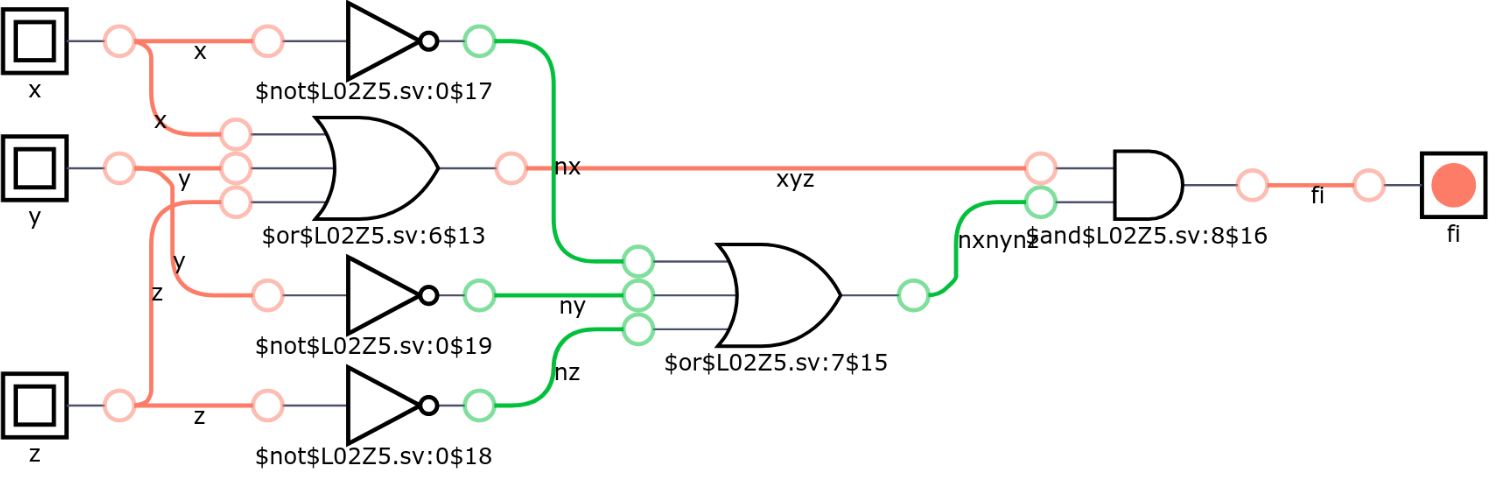
\includegraphics[scale=0.3]{./L02Z05.png}
\end{center}
\section{Zaimplementuj funkcję opisaną poniższą tabelką logiczną używając wyłącznie bramek NAND}
\begin{center}
	\begin{tabular}{|c|c|c||c|} 
	 \hline
	$x$ & $y$ & $z$ & $\Phi$\\ 
	 \hline \hline
	 0&0&0&0\\ \hline
	 0&0&1&1\\ \hline
	 0&1&0&1\\ \hline
	 0&1&1&0\\ \hline
	 1&0&0&1\\ \hline	 
	 1&0&1&0\\ \hline
	 1&1&0&0\\ \hline
	 1&1&1&1\\ \hline
	\end{tabular}\\
	$\Phi = (x+y+z)(x+\bar y + \bar z)(\bar x+y+\bar z)(x+\bar y+\bar z) = \neg{(\bar x \bar y \bar z)} \neg{( \bar x y  z)} \neg{( x \bar y z)} \neg{(x  y \bar z)}$\\
	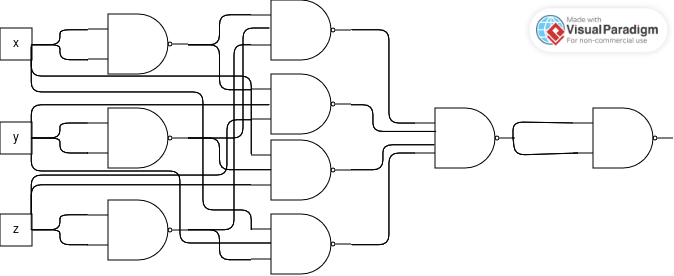
\includegraphics[scale=0.3]{./L02Z06.png}
	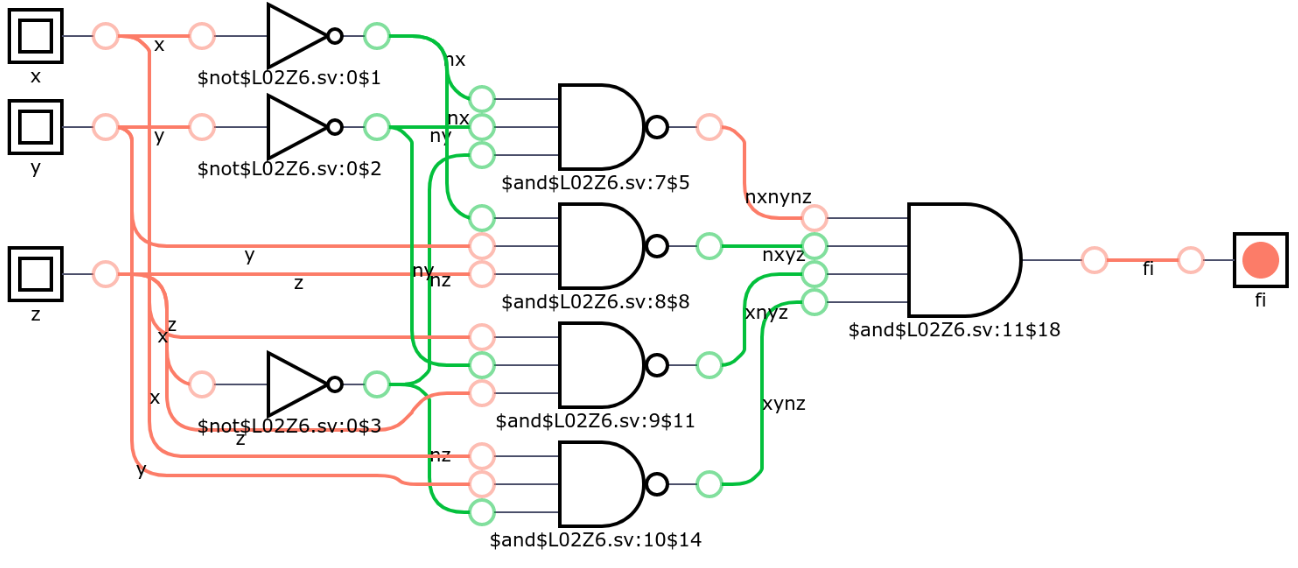
\includegraphics[scale=0.3]{./L02Z06czII.png}\\
	\textbf{można zbić o jedną negację na wyjściu}
\end{center}
\section{Napisz najmniejsze wyrażenie odpowiadające poniższej tabelce logicznej. Pamiętaj o wykorzystaniu wartości don’t care.}
\begin{center}

\begin{tabular}{|c|c|c|c||c|} 
	 \hline
	$x$ & $y$ & $z$ & $w$ & $\Phi$\\ 
	 \hline \hline
	 0&0&0&0&x\\ \hline
	 0&0&0&1&x\\ \hline
	 0&0&1&0&x\\ \hline
	 0&0&1&1&0\\ \hline
	 
	 0&1&0&0&0\\ \hline	 
	 0&1&0&1&x\\ \hline
	 0&1&1&0&0\\ \hline
	 0&1&1&1&x\\ \hline
	 
	 1&0&0&0&1\\ \hline
	 1&0&0&1&0\\ \hline
	 1&0&1&0&x\\ \hline
	 1&0&1&1&1\\ \hline
	 
	 1&1&0&0&1\\ \hline	 
	 1&1&0&1&1\\ \hline
	 1&1&1&0&x\\ \hline
	 1&1&1&1&1\\ \hline
	 \end{tabular}
	 \begin{tabular}{|c|c|c|c|c|} 
	 \hline
	xy\textbackslash zw& 00 & 01 & 11 & 10\\ 
	 \hline
	 00&x&x&0&x \\ \hline
	 01&0&\textcolor{red}{x}&\textcolor{red}{x}&0\\ \hline
	 11&\textcolor{blue}{1}&\textcolor{red}{1}&\textcolor{red}{1}\textbackslash \textcolor{orange}{1}&\textcolor{blue}{x}\textbackslash \textcolor{orange}{1} \\ \hline
	 10&\textcolor{blue}{1}&0&\textcolor{orange}{x}&\textcolor{blue}{x}\textbackslash \textcolor{orange}{x} \\ \hline
	 \end{tabular}\\
	 $\Phi = \textcolor{red}{yw}+\textcolor{blue}{x\bar{w}}+\textcolor{orange}{xz}$
\end{center}
\section{Czy w układzie odpowiadającym wyrażeniu z poprzedniego zadania może wystąpić glitch? Jeśli nie, wyjaśnij dlaczego. Jeśli tak, pokaż, jak zmodyfikować układ, aby wyeliminować glitch}
\textbf{glitch} polega na zmianie wartości zmiennej które zmienia choć nie powinno wyniku (albo odwrotnie)
mój układ nie jest odporny na to, wystarczy równocześnie zapalić w i x.\\
\begin{center}

	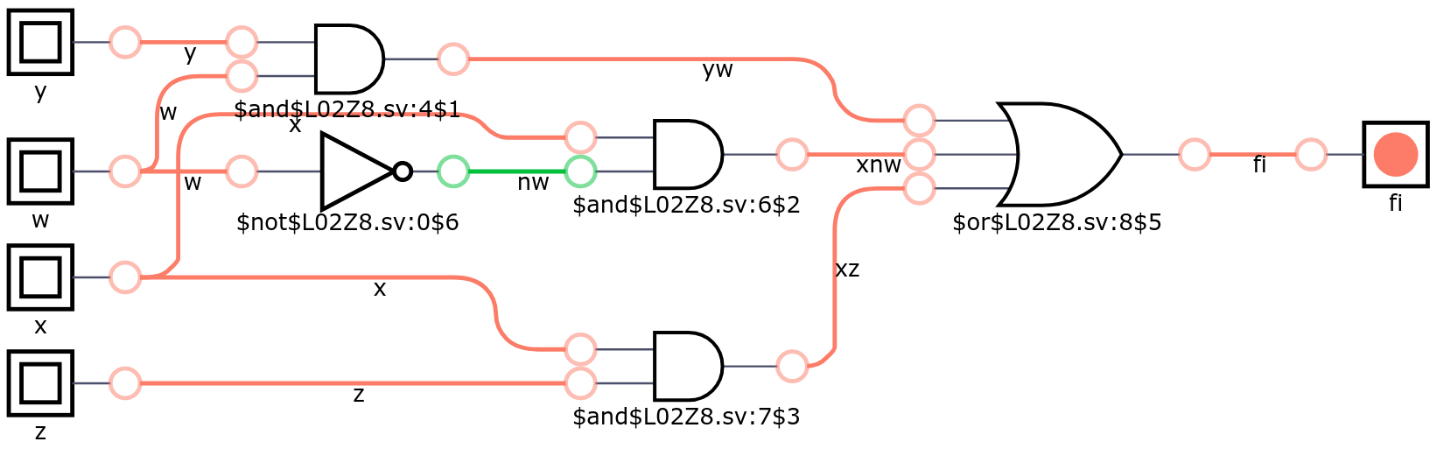
\includegraphics[scale=0.2]{./L02Z08.png}
	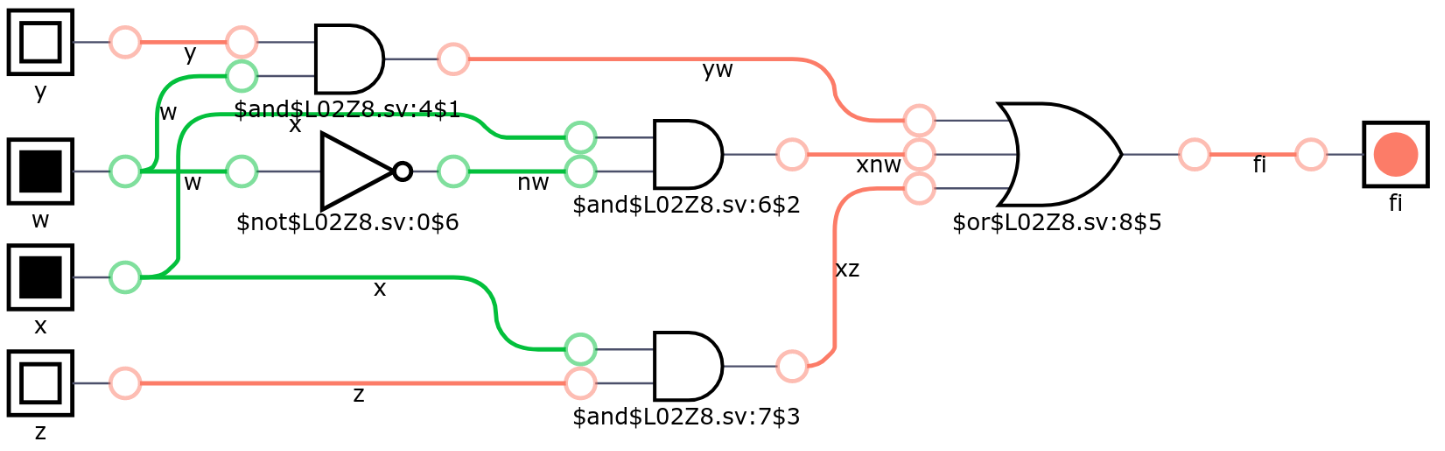
\includegraphics[scale=0.2]{./L02Z08czII.png}
\end{center}
można w inny sposób odczytać to wszystko, aby się zabezpieczyć przed glitchem:\\
\begin{center}
	 \begin{tabular}{|c|c|c|c|c|} 
	 \hline
	xy \textbackslash zw& 00 & 01 & 11 & 10\\ 
	 \hline
	 00&\textcolor{red}x&\textcolor{red}x\textbackslash \textcolor{blue}x &\textcolor{red}0&\textcolor{red}x \\ \hline
	 01&\textcolor{red}0&\textcolor{red}x&\textcolor{red}x&\textcolor{red}0\\ \hline
	 11&1&1&1&x \\ \hline
	 10&1&\textcolor{blue}0&1&x \\ \hline
	 \end{tabular}\\
	 $\Phi = \textcolor{red}{x}(\textcolor{blue}{z+y+ \bar{w}})$\\
	 warto wiedzieć, że glitche występują na "granicach" bloków o ile nie są połączone.
\end{center}

\end{document}